%
% orion2.tex -- filtered backprojection illustration
%
% (c) 2021 Prof Dr Andreas Müller, OST Ostschweizer Fachhochschule
%
\documentclass[tikz]{standalone}
\usepackage{amsmath}
\usepackage{times}
\usepackage{txfonts}
\usepackage{pgfplots}
\usepackage{csvsimple}
\usepackage{mathrsfs}
\usetikzlibrary{arrows,intersections,math}
\begin{document}
\def\skala{1}
\begin{tikzpicture}[>=latex,thick,scale=\skala]
\clip (-7,-7.5) rectangle (7,7.5);
\fill[color=black!80] (-7,-7.5) rectangle (7,7.5);

\begin{scope}[xshift=-3.6cm,yshift=4.1cm]
\node at (0,0) {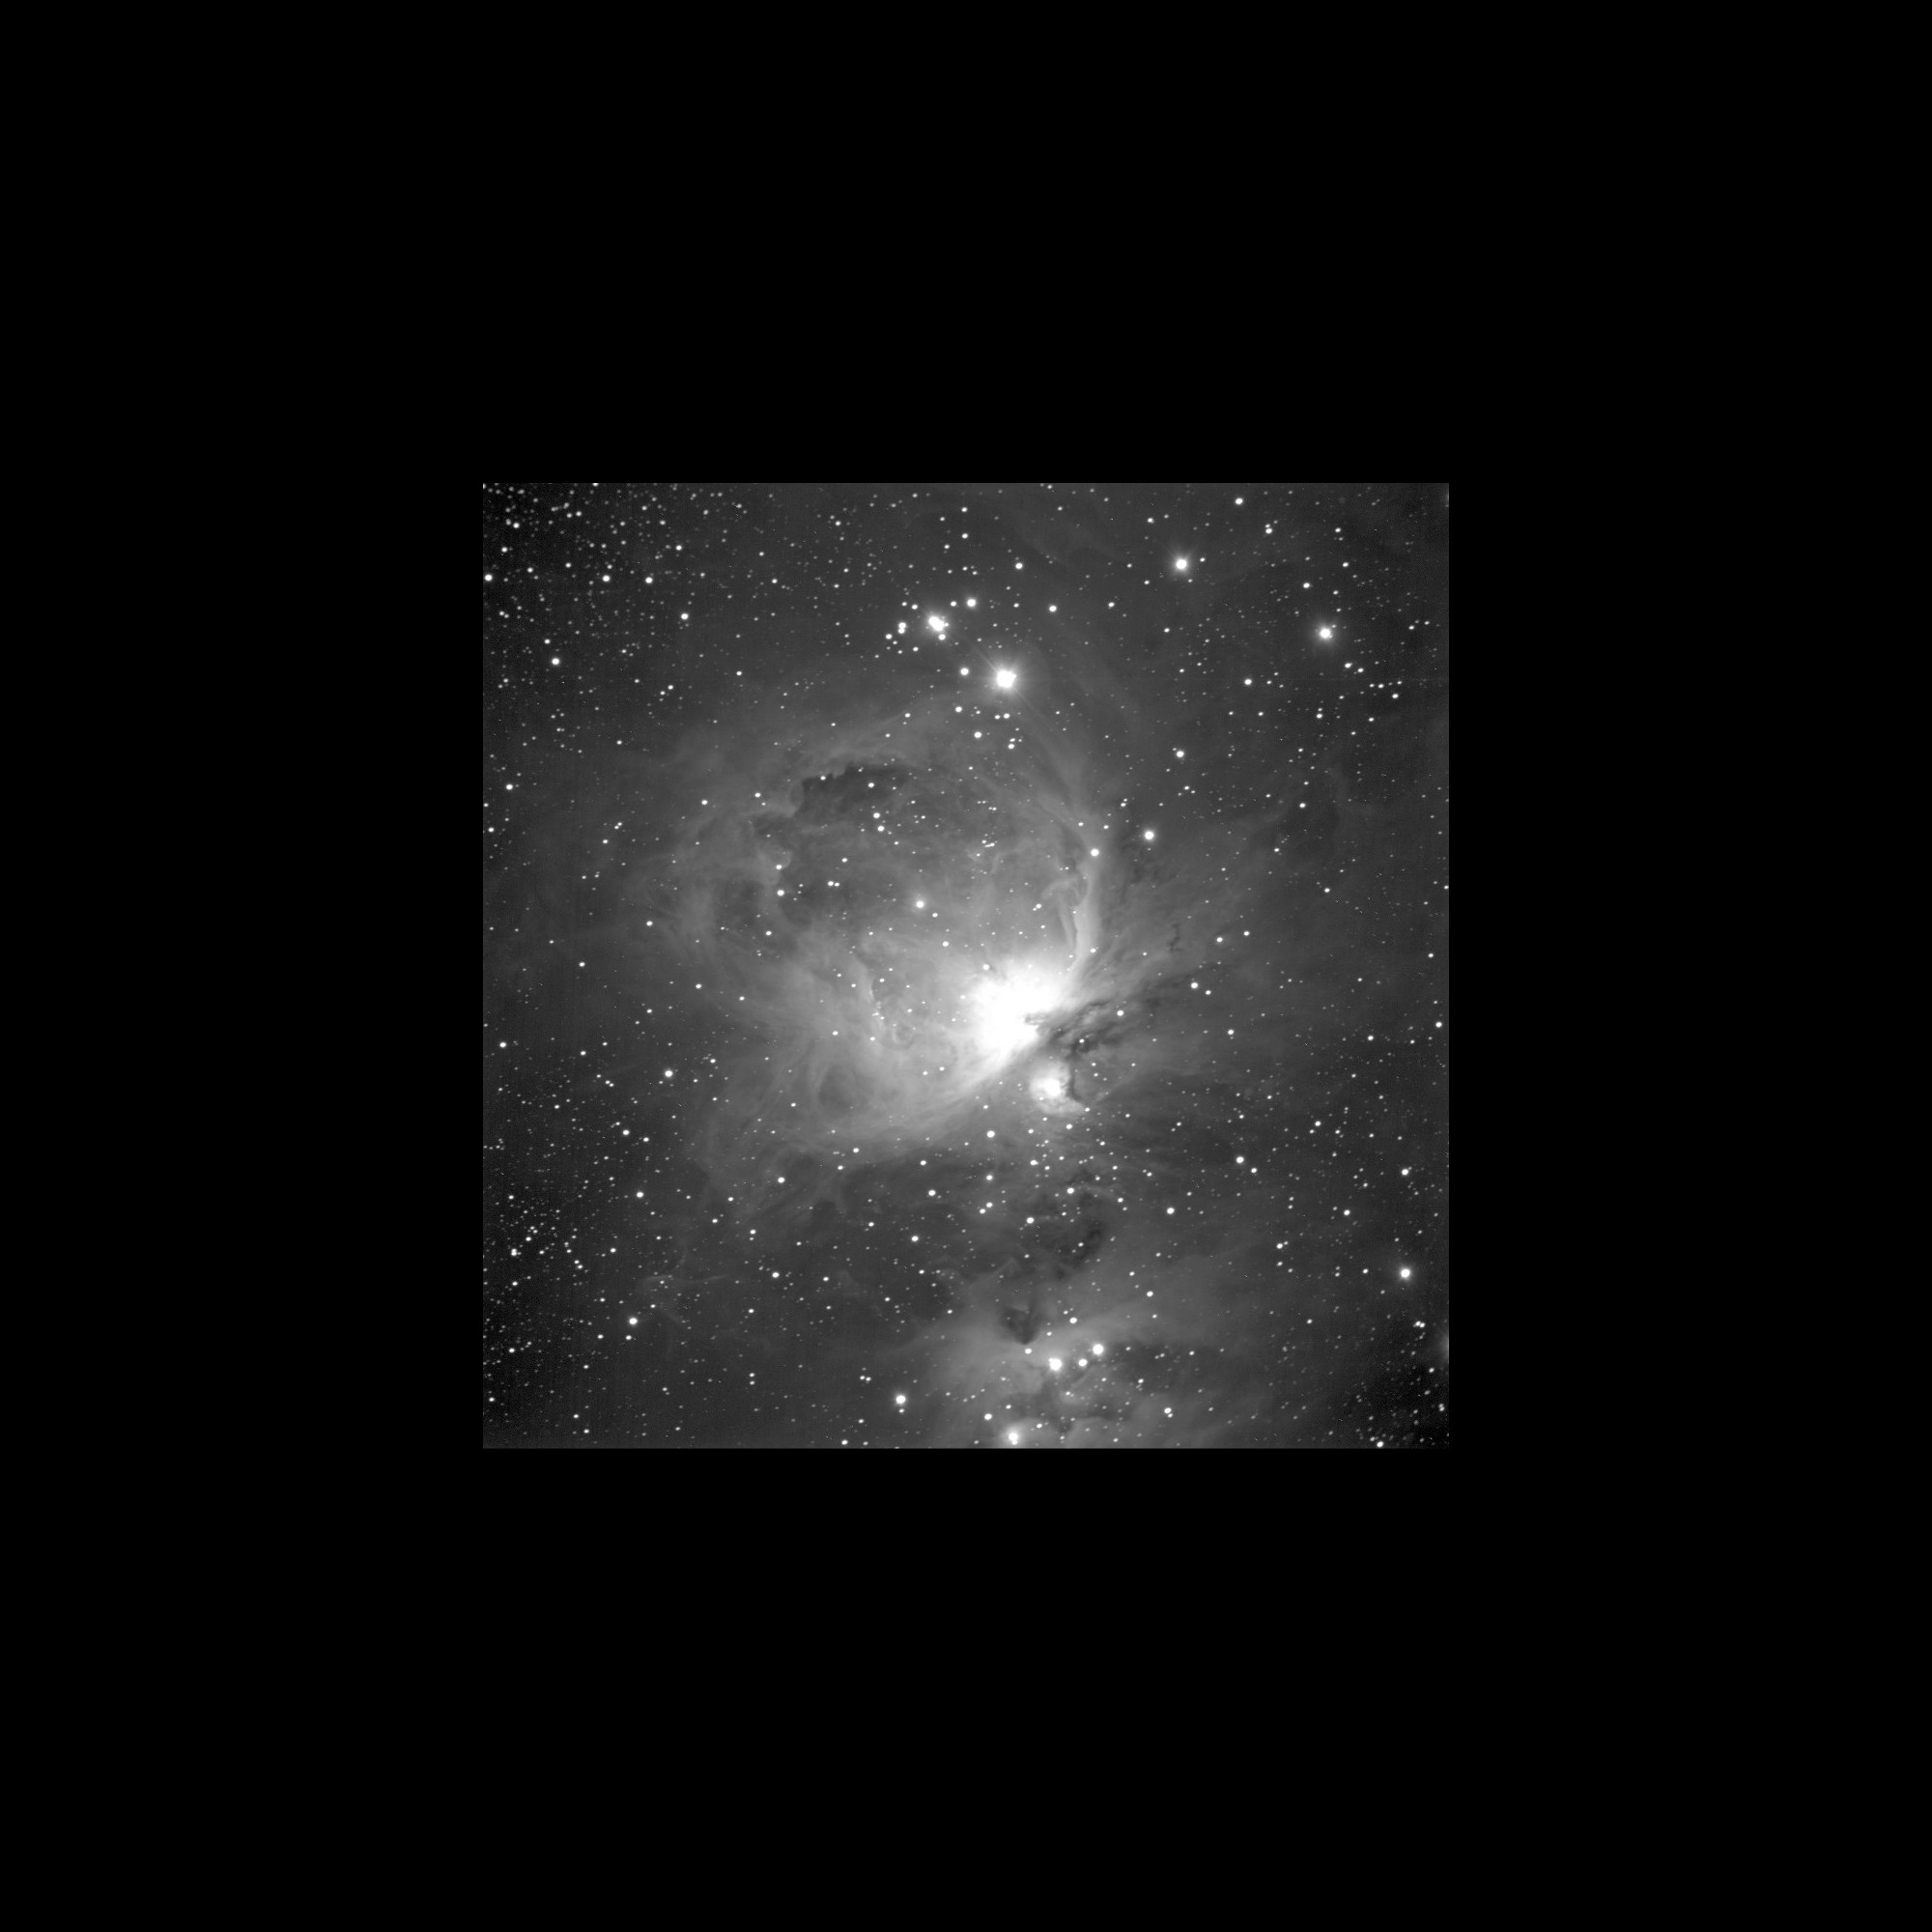
\includegraphics[width=6.8cm]{orion2.jpg}};
\node[color=white] at (-3.4,3.4) [below right] {$u(x,y)$};
\end{scope}

\begin{scope}[xshift=3.6cm,yshift=4.1cm]
\node at (0,0) {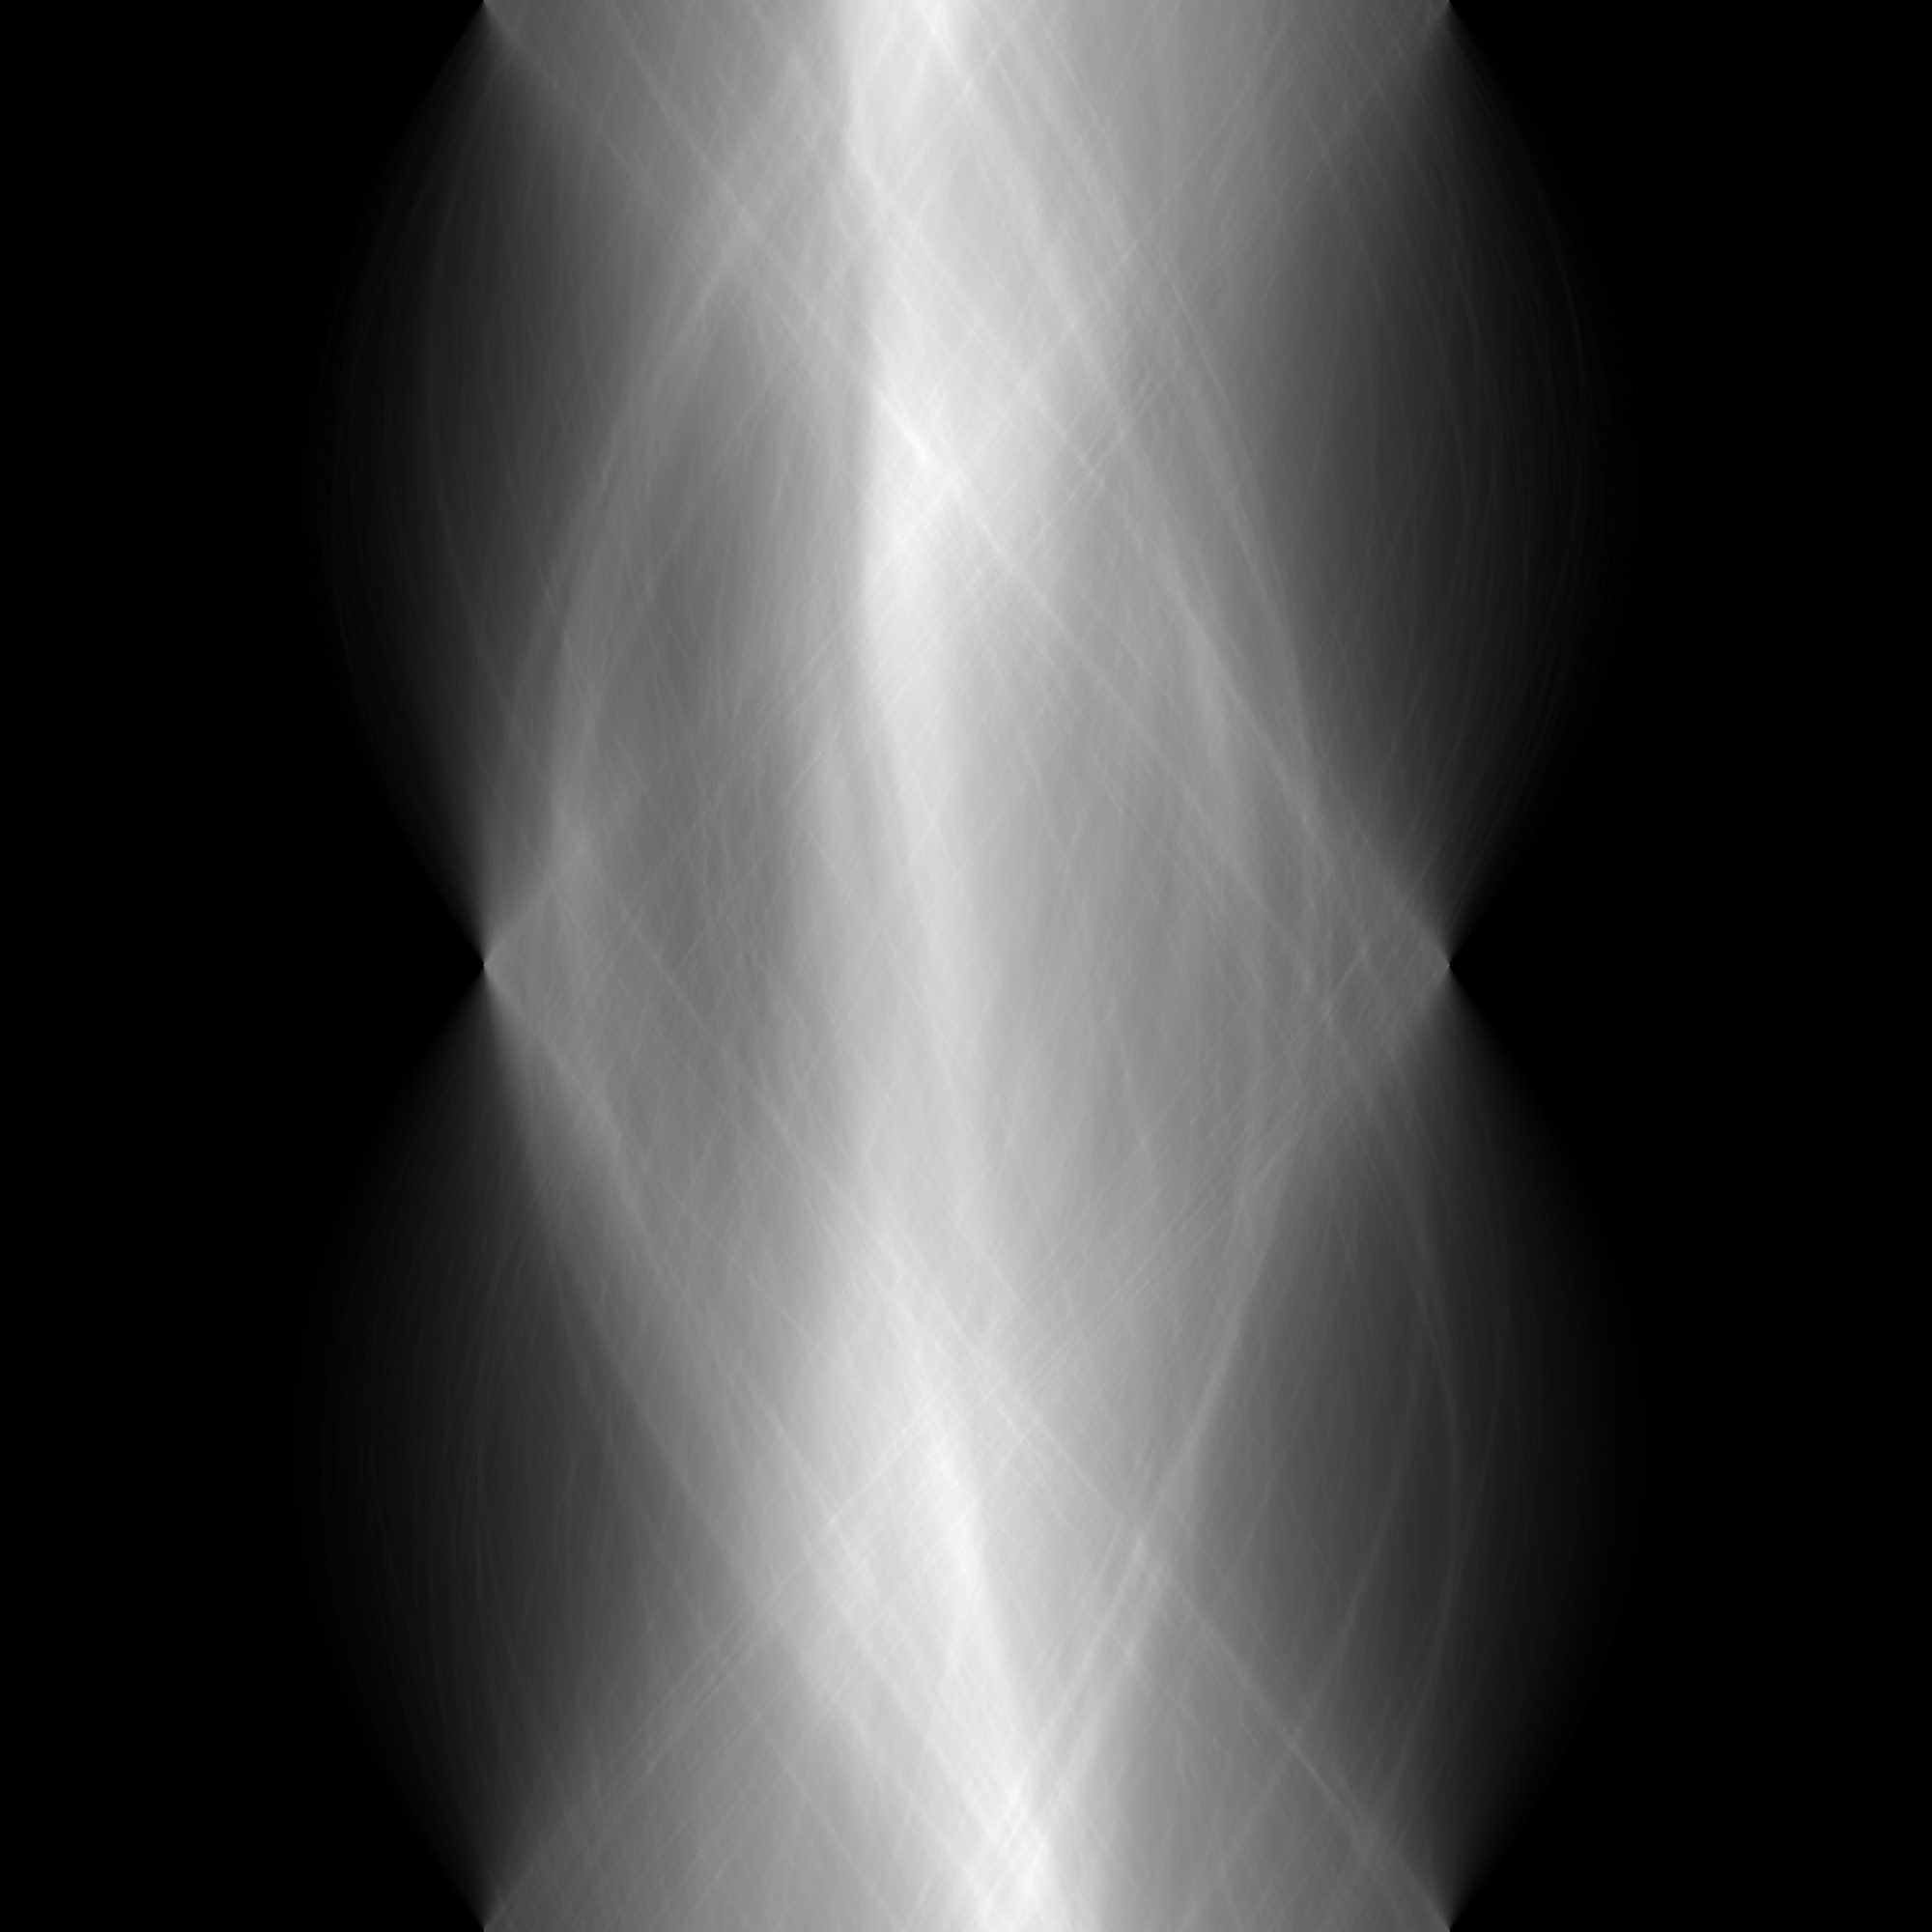
\includegraphics[width=6.8cm]{orion2-radon.jpg}};
\node[color=white] at (3.4,3.4) [below left] {$\mathscr{R}u$};
\end{scope}

\begin{scope}[xshift=3.6cm,yshift=-4.1cm]
\node at (0,0) {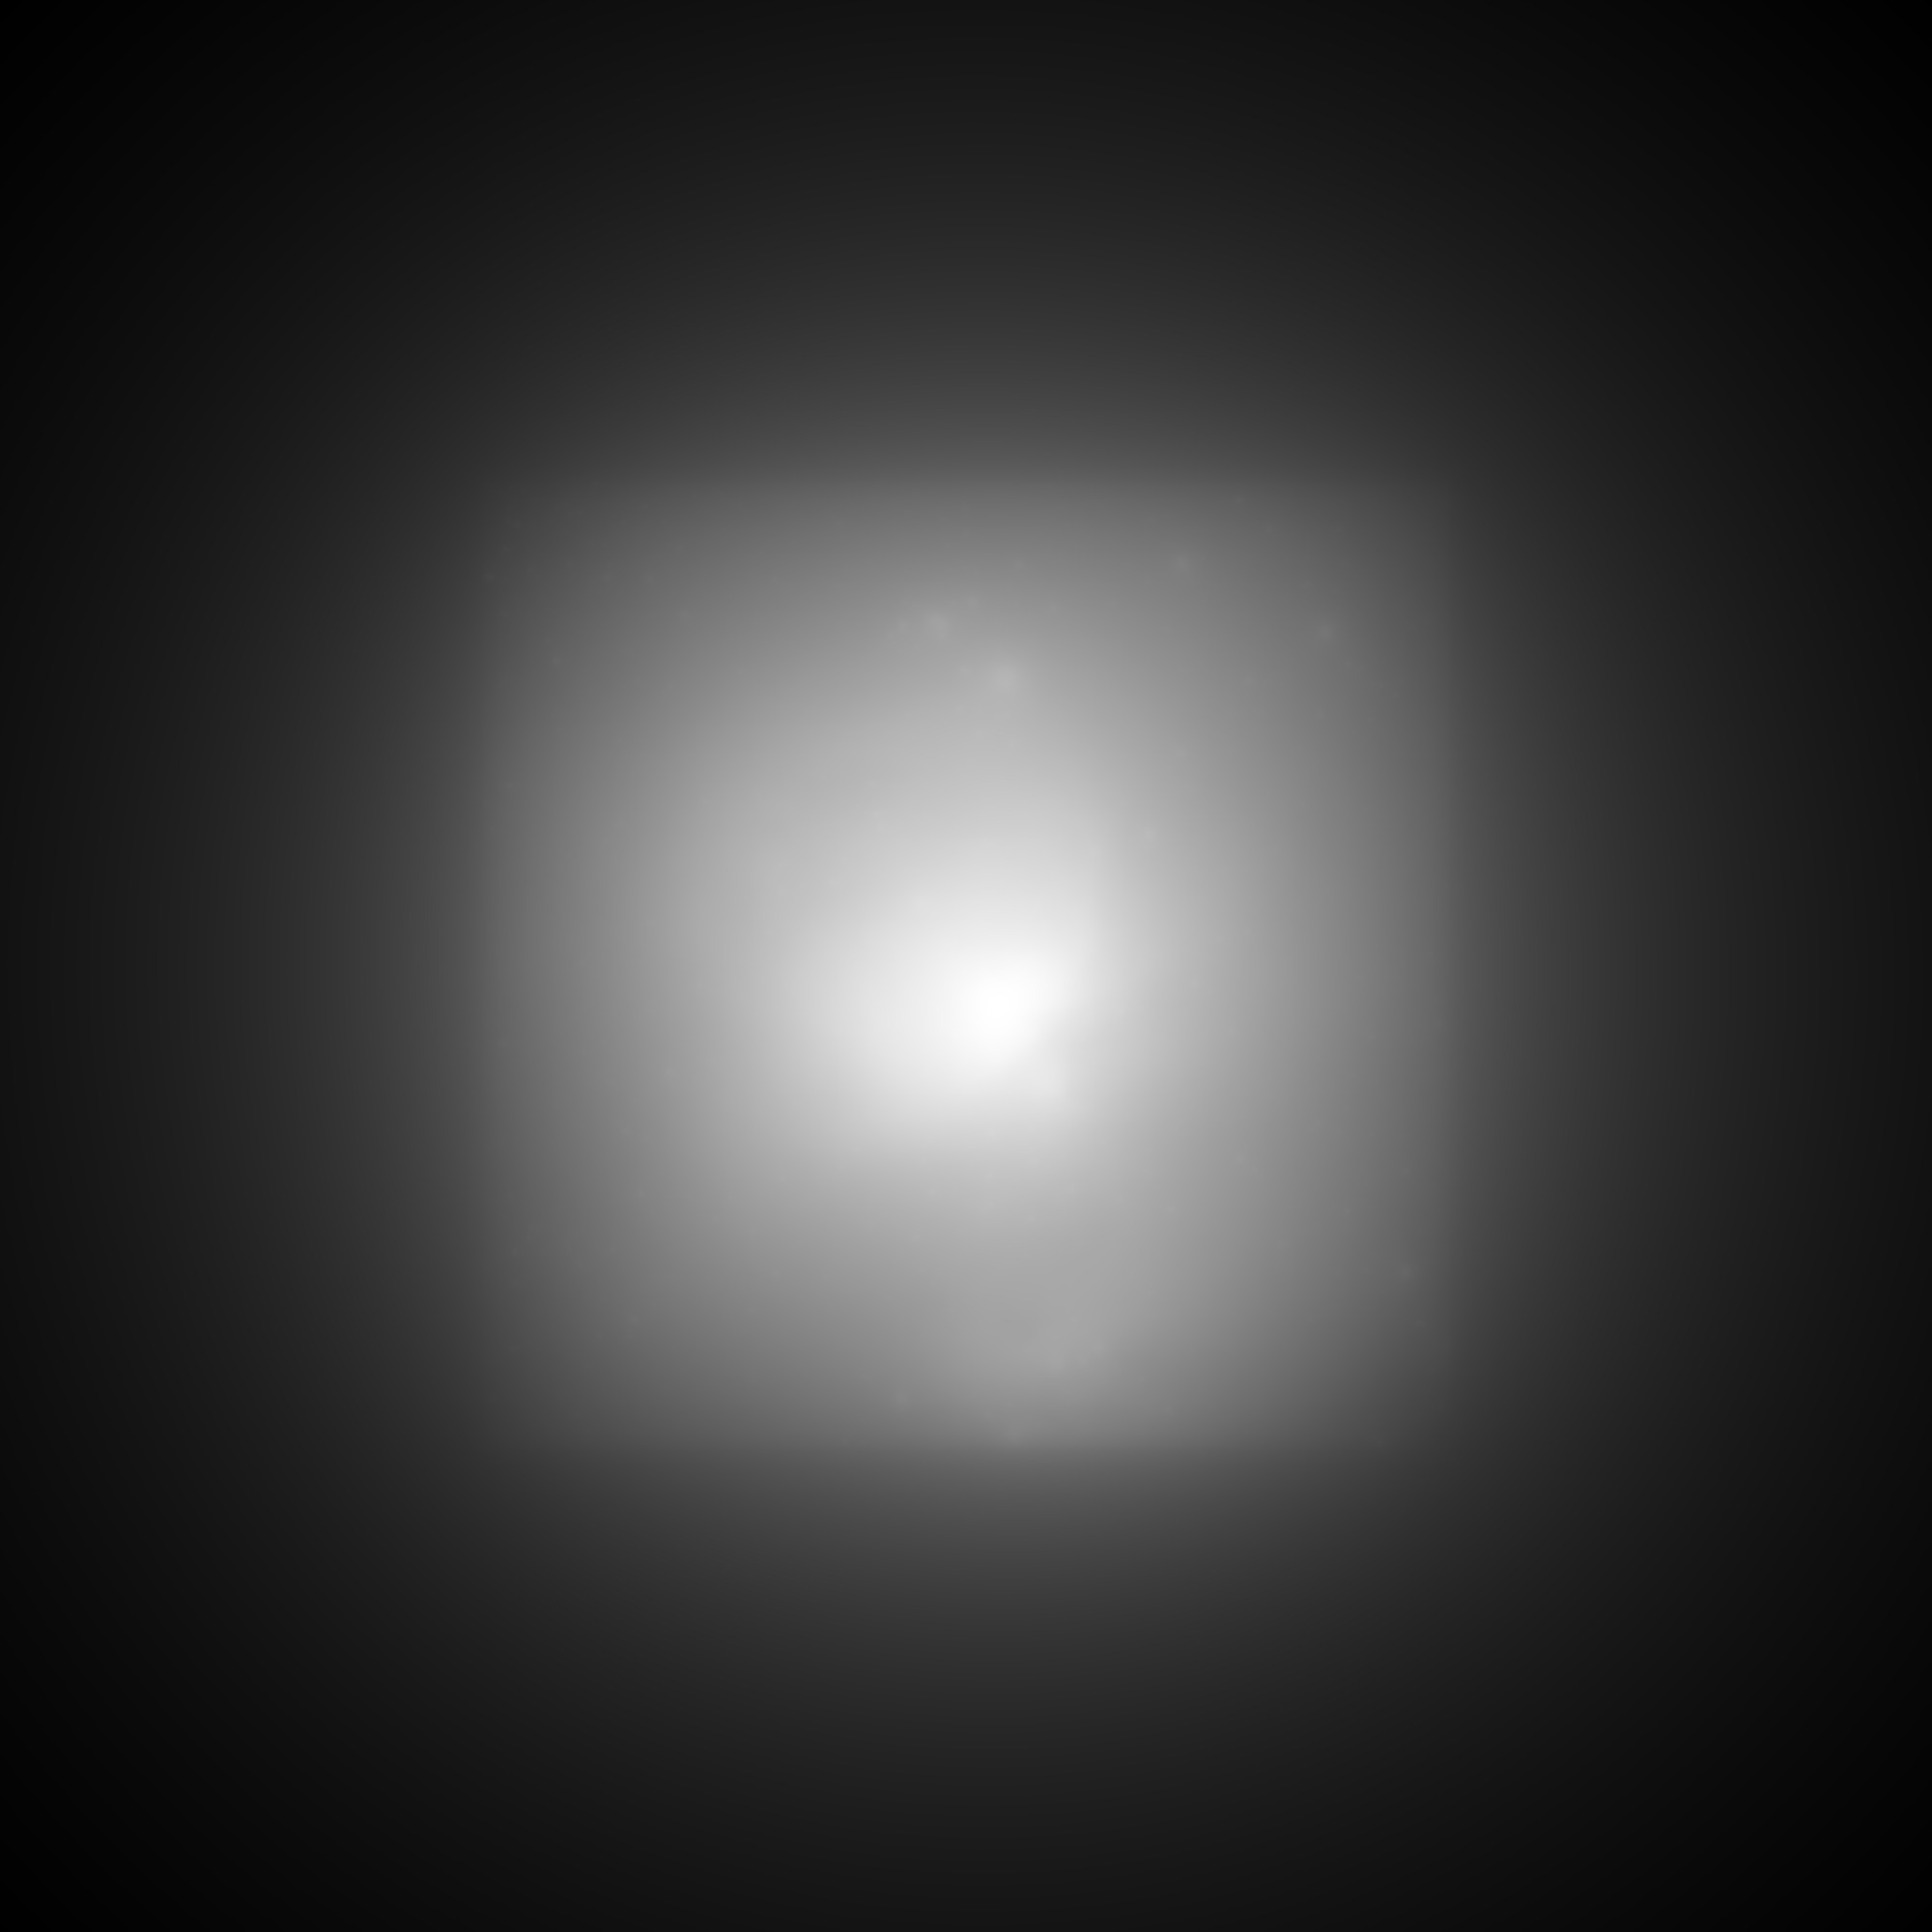
\includegraphics[width=6.8cm]{orion2-backprojection.jpg}};
\node[color=white] at (3.4,-3.4) [above left] {$\mathscr{R}^*\mathscr{R}u$};
\end{scope}

\begin{scope}[xshift=-3.6cm,yshift=-4.1cm]
\node at (0,0) {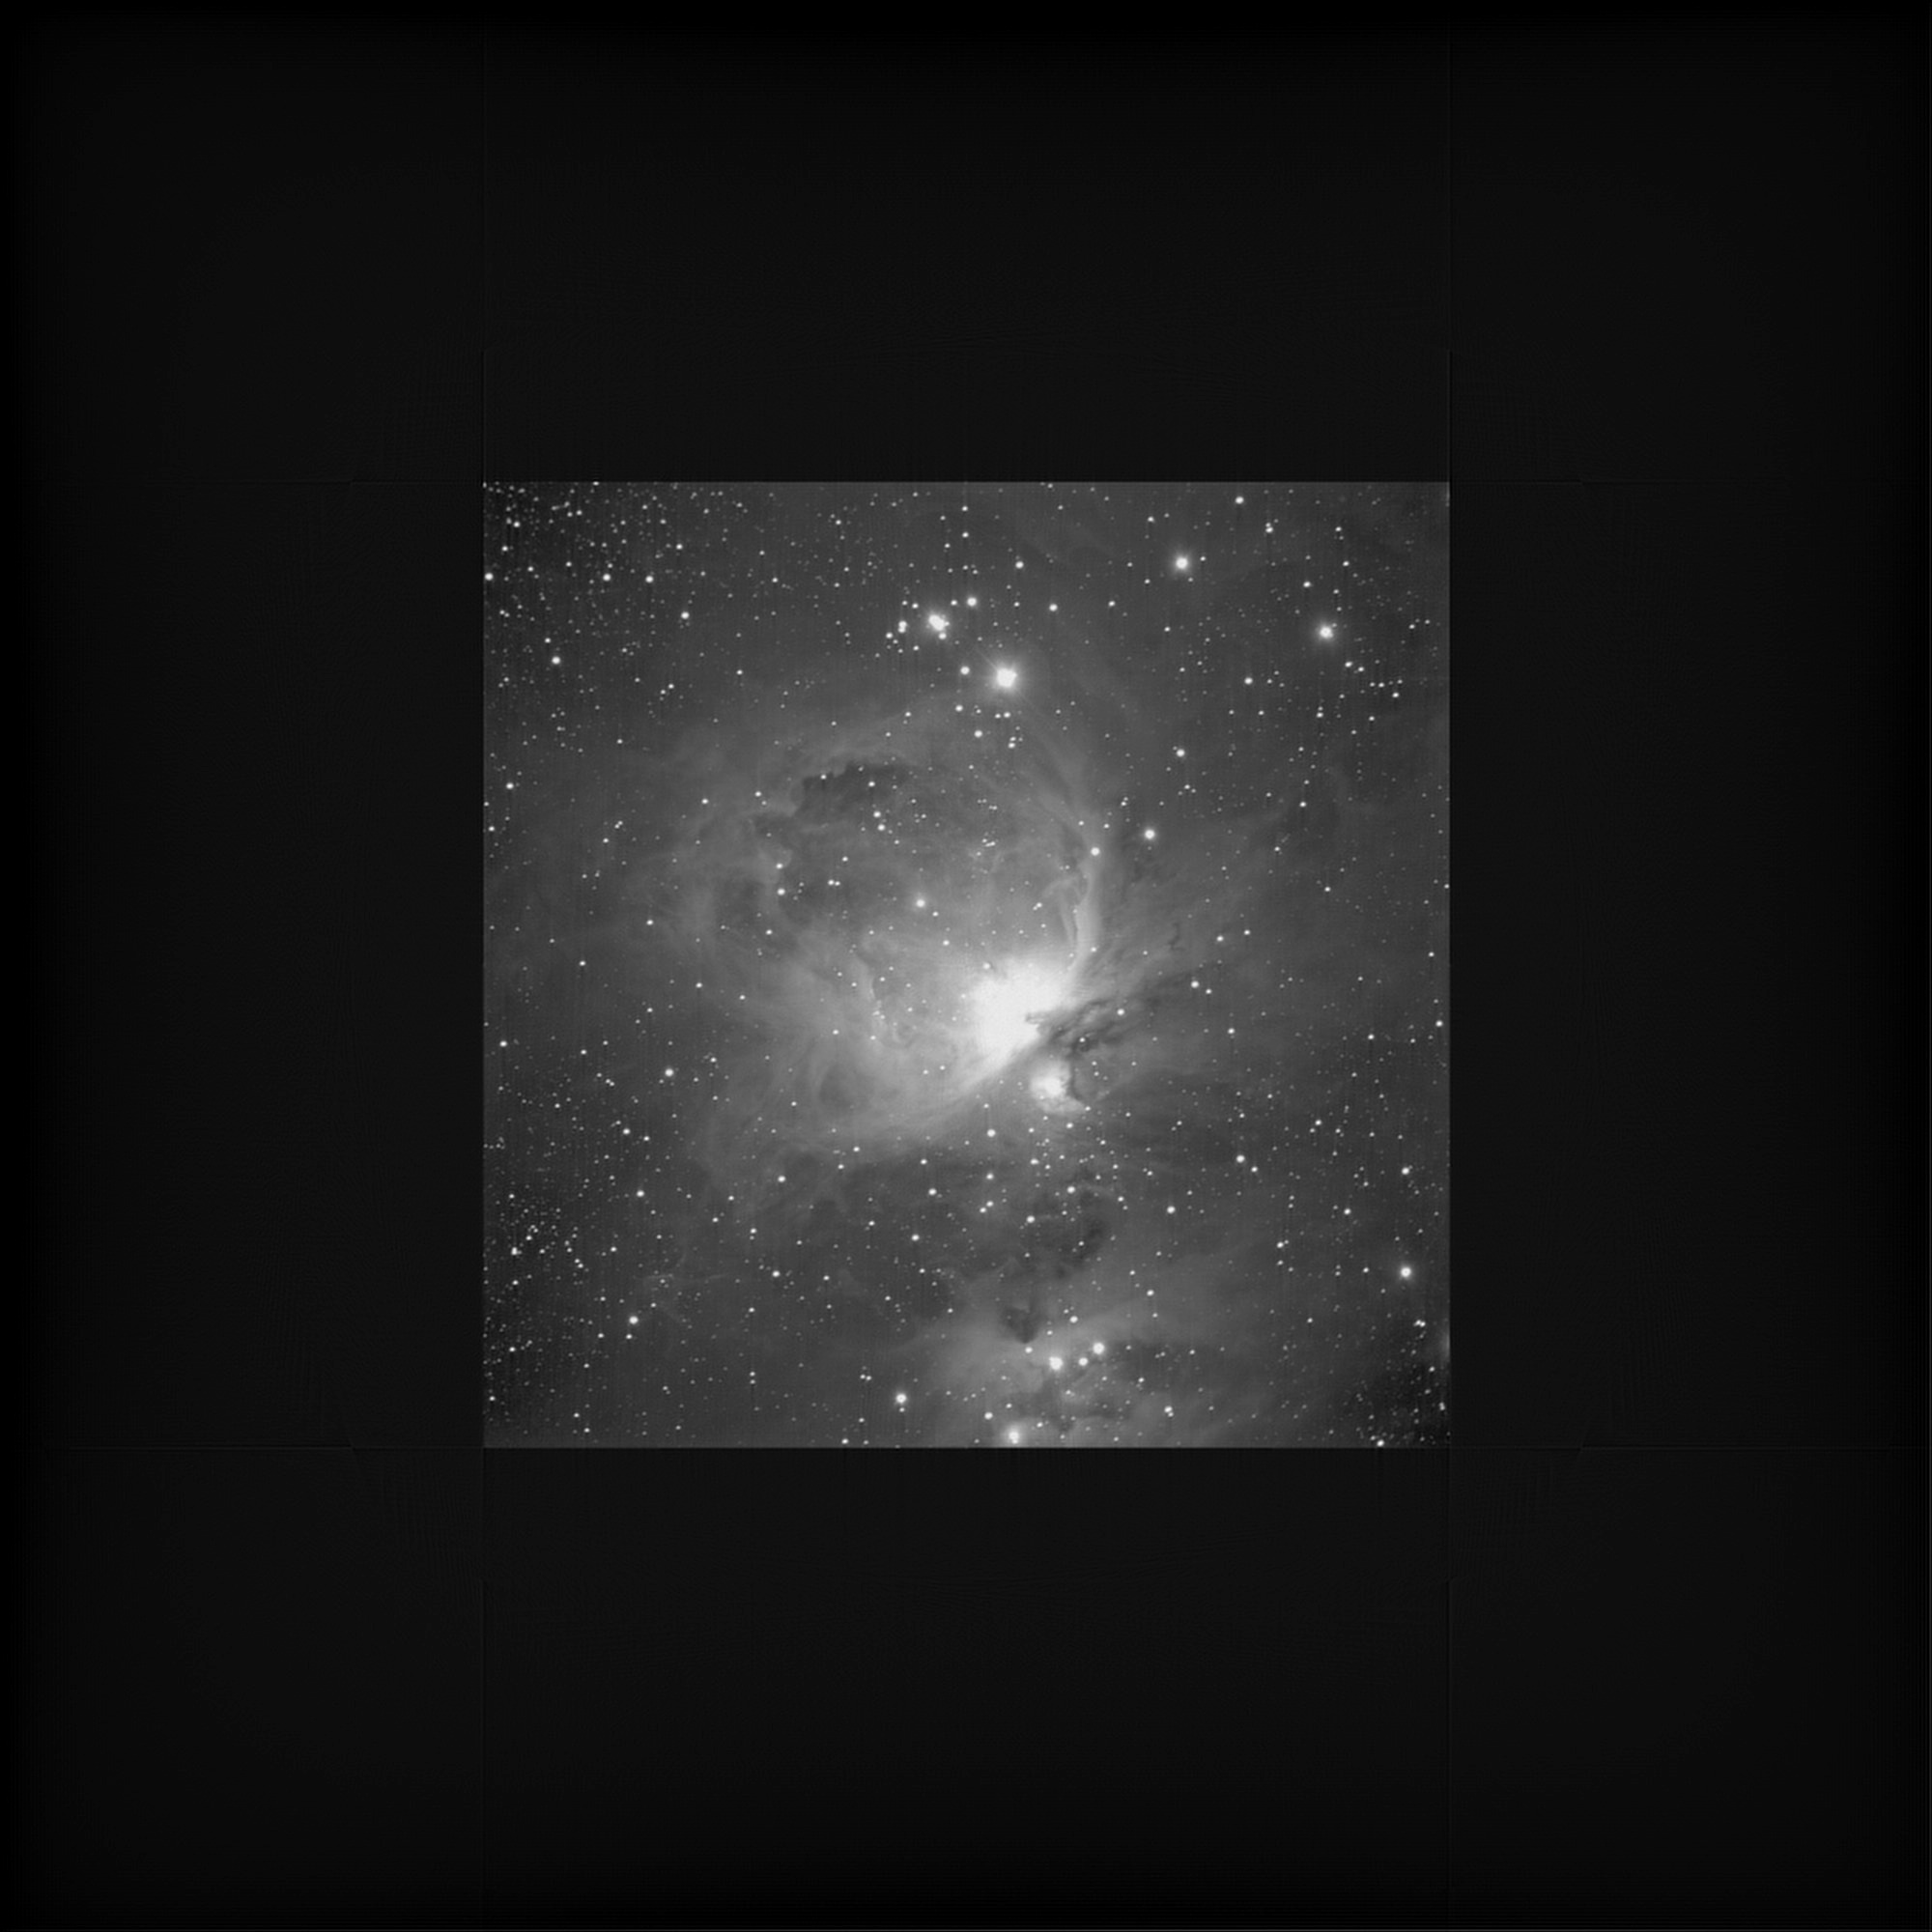
\includegraphics[width=6.8cm]{orion2-filtered-backprojection-corrected.jpg}};
\node[color=white] at (-3.4,-3.4) [above right] {$\mathscr{R}^*\mathscr{F}_r^{-1}|r|\mathscr{F}_r\mathscr{R}u$};
\end{scope}

\draw[->,color=white] (-1,4.0) -- (1,4.0);
\node[color=white] at (0,4.0) [above] {$\mathscr{R}\mathstrut$};

\draw[->,color=white] (3.5,1) -- (3.5,-1);
\node[color=white] at (3.5,0) [right] {$\mathscr{R}^*\mathstrut$};

\draw[->,color=white] (0.7,1.1) -- (-0.7,-1.1);
\node[color=white] at (0,0) [left]
	{$\mathscr{R}^*\mathscr{F}^{-1}_r|r|\mathscr{F}_r\mathstrut$};

\def\d{0.03}
\draw[color=white] ({-3.5+\d},-1) to[out=82,in=-98] ({-3.5+\d},1);
\draw[color=white] ({-3.5-\d},-1) to[out=82,in=-98] ({-3.5-\d},1);

\end{tikzpicture}
\end{document}

